\documentclass{article}
\usepackage{tikz, comment}
\usepackage{pifont}
\usepackage{fontspec, pgfplots}
\usetikzlibrary{arrows, decorations.markings, decorations.pathreplacing}
\begin{comment}
:Title: Not defined yet
:Tags: equation of a line;focus of a parabola;two intercept form for the equation of a line;inverse variation, inverse proportion , inversely proportional ;perimeter
:Prob: 0.5304;0.4583;0.4562;0.4561;0.4557
:Author: Prof.Hu Ji-shan, HKUST
:Slug: No name yet

Description Here.........
\end{comment}
\begin{document}\centering

\newcommand{\AxisRotator}[1][rotate=0]{%
\tikz [x=0.25cm,y=0.60cm,line width=.2ex,-stealth,#1] \draw (0,0) arc (-270:-45:1 and 1);%
}

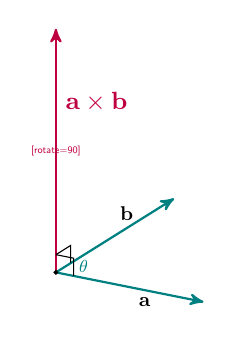
\begin{tikzpicture}[>=latex,xscale=.5*1.5, yscale=.5*1.5][font=\sf\small] 

\draw[teal, thick, ->, >=stealth'] (0, 0) -- (2.5, -0.5)node[black, below, midway, pos=0.6, xshift=0, yshift=0, scale=0.8]{${\bf a}$};

\draw[teal, thick, ->, >=stealth'] (0, 0) -- (2, 1.25)node[black, above, midway, pos=0.6, xshift=0, yshift=0, scale=0.8]{${\bf b}$};

\draw[purple, thick, ->, >=stealth'] (0, 0) -- (0, 4.125)node[right, pos= 0.7] {\small $\bf a \times b$} node [solid, midway, pos=0.5, scale=0.4]{\AxisRotator[rotate=90]} ;

\draw (0, {0+0.3})--({0.25/2*2}, {0.3+0.25/2*1.25})--({0.25/2*2}, {0.25/2*1.25});
\draw (0, {0+0.3})--({0.3/2.5*2.5}, {0.3+0.3/2.5*(-0.5)})--({0.3/2.5*2.5}, {0.3/2.5*(-0.5)});

\node[teal, xshift=10, yshift=2, scale=0.7] at (0, 0) {$\theta$};

\draw[fill] (0, 0) circle(0.03);

\end{tikzpicture}
\end{document}